\section{Electrostática}

La teoría electromagnética clásica estudia los fenómenos eléctricos y magnéticos, \hl{describiendo} sus características y las \hl{leyes} que los gobiernan.  

Cuando hablamos de \textbf{teoría clásica}, nos referimos a que se basa en la mecánica clásica de Isaac Newton. En esta mecánica se utilizan conceptos como partículas, trayectorias y las leyes del movimiento de Newton. De manera similar, en la teoría electromagnética se aplican estos conceptos a las cargas eléctricas y a los campos eléctricos y magnéticos. Es decir, en lugar de hablar solo de partículas y fuerzas mecánicas, hablaremos de \textbf{partículas cargadas, fuerzas eléctricas y campos electromagnéticos}.  

El electromagnetismo es una \hl{teoría de campos}. Por ejemplo, una \textbf{carga eléctrica} genera un \textbf{campo eléctrico} a su alrededor, mientras que un \textbf{imán} produce un \textbf{campo magnético} en el espacio que lo rodea. Estos campos son \hl{perturbaciones en el espacio} que afectan a otras cargas o imanes cercanos y pueden describirse matemáticamente.  

A lo largo de la historia, se ha comprobado que existen dos tipos de carga eléctrica: \textbf{positiva} y \textbf{negativa}. Las cargas del mismo tipo se repelen, mientras que las de signos opuestos se atraen.  

\subsection{Carga y Materia}

Todo lo que nos rodea, como una pelota, el aire, una planta o nuestro propio cuerpo, está formado por \textbf{átomos}. Los átomos, a su vez, están compuestos por tres tipos de partículas: \textbf{protones, neutrones y electrones}. Los protones y neutrones se encuentran en el núcleo del átomo, mientras que los electrones se mueven alrededor en la corteza. Los protones tienen \hl{carga positiva}, los electrones \hl{carga negativa}, y los neutrones no tienen carga. 

\begin{figure}[ht]
    \centering
    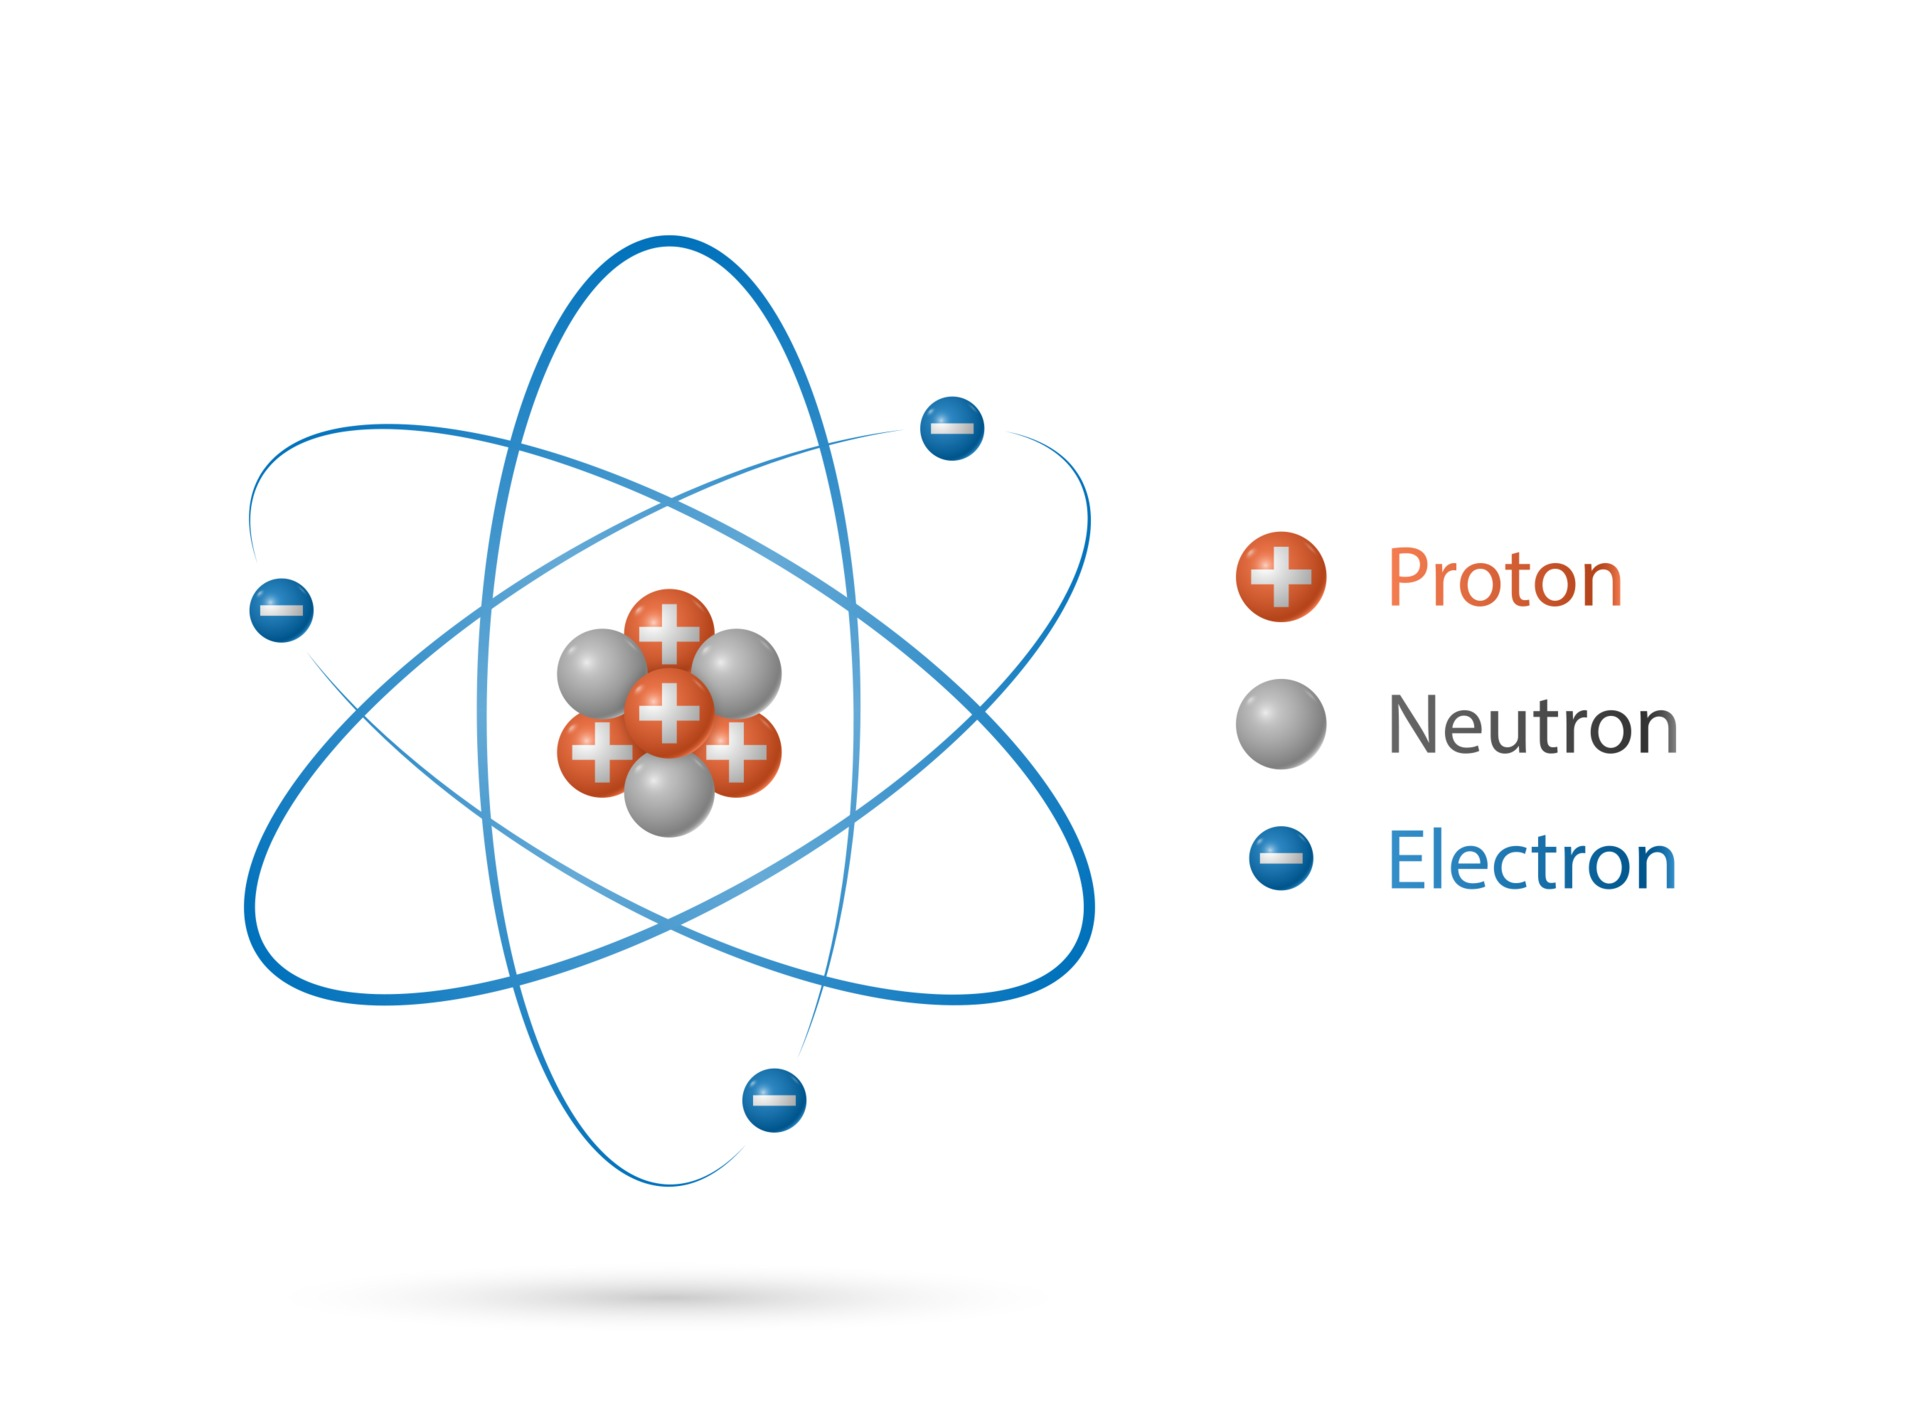
\includegraphics[width=0.4\textwidth]{images/atom_struct.jpg}
    \caption{Estructura básica de un átomo.}
    \label{fig:atom_struct}
\end{figure}

Esta estructura corresponde a un \textbf{modelo atómico}, que es una representación que nos ayuda a entender cómo está compuesto un átomo y cómo se comporta. A lo largo del tiempo han existido distintos modelos atómicos, pero uno de los más conocidos es el \textbf{modelo de Bohr}. Según este modelo, los electrones giran alrededor del núcleo en \textbf{órbitas circulares}, cada una con un nivel de energía específico. Cuando un electrón cambia de órbita, absorbe o emite energía en forma de luz.

La carga elemental \colorbox{highlight}{\( e \)} es la \textbf{cantidad más pequeña de carga eléctrica libre que se conoce en la naturaleza}. Es la carga que poseen los protones y electrones, pero con signo opuesto:

\begin{itemize}
    \item \textbf{Electrón}: \( -e = -1.602 \times 10^{-19} \) C (coulombs)
    \item \textbf{Protón}: \( +e = 1.602 \times 10^{-19} \) C
\end{itemize}

La carga elemental es fundamental porque todas las cargas eléctricas observadas en la naturaleza son \textbf{múltiplos enteros de \( e \)}. Es decir, cualquier carga presente en un objeto es el resultado de un exceso o déficit de electrones. Este principio se conoce como la \textbf{ley de conservación de la carga eléctrica}, y establece que la carga eléctrica \textbf{no se crea ni se destruye}, solo se transfiere de un cuerpo a otro.  

Los objetos tienen carga debido a la presencia de \textbf{electrones y protones}. Un objeto es eléctricamente neutro cuando tiene igual número de ambos. Si un objeto adquiere carga negativa, significa que ha \textbf{ganado electrones}, y si adquiere carga positiva, significa que ha \textbf{perdido electrones}. Cuando un objeto se carga, no se están creando nuevas cargas, sino que \textbf{se están moviendo electrones} de un cuerpo a otro. Por ejemplo: en la \textbf{electrización por frotamiento}, un material transfiere electrones a otro, dejando uno cargado positivamente y el otro negativamente. En la \textbf{inducción}, un objeto cargado puede redistribuir las cargas en otro sin tocarlo, pero sin cambiar la cantidad total de carga en el sistema.

En otras palabras, la carga eléctrica siempre se conserva porque \textbf{los electrones y protones no se destruyen en procesos normales}, solo cambian de ubicación dentro de un sistema.

\colorbox{highlight}{Denominaremos con la letra \( Q \) o \( q \) a la carga eléctrica de un objeto.} La carga se mide en \textbf{coulombs (C)}. Un coulomb es una cantidad de carga muy grande, por lo que en la práctica se utilizan submúltiplos como el \textbf{millicoulomb (mC)} o el \textbf{microcoulomb (\( \mu \text{C} \))}.

\subsection{Fuerza y campo eléctrico}

\subsubsection{Ley de Coulomb}

La electrostática estudia las cargas eléctricas en \hl{\textbf{reposo}}. La ley de Coulomb establece que \textbf{la fuerza entre dos cargas puntuales} es:

\begin{equation}
    F = k_e \frac{\abs{q_1} \cdot \abs{q_2}}{r^2}
    \label{eq:ley_coulomb}
\end{equation}

donde:

\begin{itemize}
    \item \( k_e \) es la constante de Coulomb: \( 8.9876 \times 10^9 \, \frac{\si{\newton\meter\squared}}{\si{\coulomb\squared}} \).
    \begin{itemize}
        \item \( k_e \) se obtiene de  \( \frac{1}{4\pi\epsilon_0} \) y,
        \item \( \epsilon_0 \) es la permitividad del vacío: \( 8.85 \times 10^{-12} \,\frac{\si{\coulomb\squared}}{\si{\newton\meter\squared}} \)
    \end{itemize}
    \item \( q_1 \) y \( q_2 \) son las cargas.
    \item \( r \) es la distancia entre las cargas.
\end{itemize}

Es muy importante notar que la \textbf{Ley de Coulomb} \eqref{eq:ley_coulomb} se aplica estrictamente a \hl{cargas puntuales}, es decir, cargas que se consideran concentradas en un solo punto sin dimensiones espaciales. En la ecuación anterior \eqref{eq:ley_coulomb}, se obtiene la magnitud de la fuerza eléctrica. La expresión vectorial de la fuerza eléctrica es:

\begin{equation}
    \vec{F}_e = k_e \frac{|q_1 q_2|}{r^2} \hat{r}
    \label{eq:ley_coulomb_vectorial}
\end{equation}

donde:
\begin{itemize}
    \item \( \vec{F}_e \) es el vector fuerza eléctrica entre dos cargas puntuales \( q_1 \) y \( q_2 \)
    \item \( \hat{r} \) es el vector unitario en la dirección que une ambas cargas.
\end{itemize}

Esto es importante tenerlo en cuenta ya que si se quiere saber la fuerza total sobre una carga \( q \) debido a varias cargas, se debe sumar vectorialmente las fuerzas individuales. La fuerza total sobre una carga \( q \) debido a un conjunto de cargas \( Q_i \) es:

\begin{equation}
    \vec{F} = \sum_i k \frac{|q \cdot Q_i|}{r_i^2} \hat{\mathbf{r_i}}
    \label{eq:ley_coulomb_vectorial_suma}
\end{equation}

\subsubsection{Cargas eléctricas}

La \textbf{carga eléctrica} es una propiedad fundamental de la materia que determina la interacción electromagnética entre partículas. Se trata de una magnitud escalar que puede ser de dos tipos: \textbf{positiva} o \textbf{negativa}. Las partículas con carga del mismo signo se repelen, mientras que las de signo opuesto se atraen.

La unidad de carga eléctrica en el \textbf{Sistema Internacional (SI)} es el \textbf{coulomb (\( \si{coulomb} \))}. La carga elemental está representada por la carga del electrón (\( -e = -1.602 \times 10^{-19} \si{coulomb} \)) y la del protón (\( e = +1.602 \times 10^{-19} \si{coulomb} \)).

\begin{center}
    \setlength{\arrayrulewidth}{1pt}  % Grosor de líneas
    \renewcommand{\arraystretch}{1.3} % Espaciado vertical
    \arrayrulecolor{gray} % Color de líneas

    \begin{tabular}{ c c c }
        \hline
        \rowcolor{asparagus!30}
        \textbf{Partícula}  & \textbf{Carga (\si{C})}           & \textbf{Masa (\si{kg})}   \\ \hline
        Electrón (e)        & \(-e = -1.602 \times 10^{-19}\)   & \(9.109 \times 10^{-31}\) \\
        Protón (p)          & \(+e = +1.602 \times 10^{-19}\)   & \(1.672 \times 10^{-27}\) \\
        Neutrón (n)         & \(0\)                             & \(1.675 \times 10^{-27}\) \\ \hline
    \end{tabular}
\end{center}

\subsubsection{Campo eléctrico}

Para entender la definición del campo eléctrico desde el principio, debemos pensar en cómo se conceptualiza la interacción entre cargas eléctricas y en la necesidad de definir una propiedad del espacio que describa esta interacción.

Sabemos que las cargas eléctricas ejercen fuerzas unas sobre otras. Experimentalmente, se observa que cargas del mismo signo se repelen y cargas de signo opuesto se atraen. Esta interacción fue formulada matemáticamente por la Ley de Coulomb \eqref{eq:ley_coulomb_vectorial}, sin embargo, esta ley solo nos dice cómo una carga afecta a otra en particular, pero no describe una propiedad del espacio en sí. Aquí es donde se introduce el concepto de \textbf{campo eléctrico}.

\begin{figure}[ht]
    \centering
    
\includegraphics[width=0.4\textwidth]{images/field_concept.png}
    \caption{Concepto de campo eléctrico.}
    \label{fig:concepto_campo_electrico}
\end{figure}

En lugar de pensar que una carga actúa instantáneamente sobre otra, se puede imaginar que una carga genera algo en el espacio a su alrededor que luego interactúa con otras cargas. Este ``algo'' es el \textbf{campo eléctrico}. La idea es la siguiente:

\begin{enumerate}
    \item Una carga fuente \( Q \) modifica el espacio circundante.
    \item Cualquier otra carga \( q \) que se coloque en ese espacio experimentará una fuerza debido a esta modificación.
    \item Para cuantificar esa modificación, definimos el campo eléctrico como la \textbf{fuerza por unidad de carga de prueba}.
\end{enumerate}

\paragraph{Idea conceptual del campo eléctrico}

Bueno, ¿qué es el campo eléctrico? Según la descripción previa, el campo eléctrico es una propiedad del espacio que rodea a una carga eléctrica capaz de interactuar con otras cargas. Veamos un ejemplo de esto para entenderlo mejor.

Supongamos que tenemos tres cargas eléctricas de distinto valor ubicadas en tres lugares distintos. Todas estas cargas están fijas en su posición y no pueden moverse. 

\begin{figure}[ht]
    \centering
    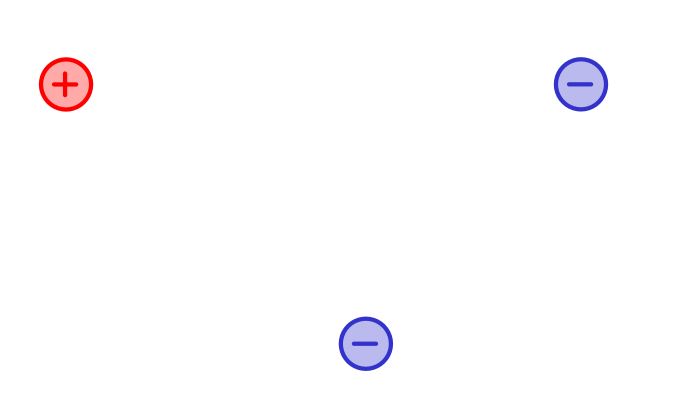
\includegraphics[width=0.5\textwidth]{images/field_ex_1.png}
    \caption{tres cargas fijas en el espacio.}
    \label{fig:campo_electrico_ejemplo_1}
\end{figure}

Ahora tomamos una cuarta carga, la colocamos en el centro de las tres cargas y la soltamos ¿Qué le pasaría? La carga sería empujada hacia algún lugar, ya que, experimentará una fuerza debido a la interacción con las otras cargas. Ya sabemos que las cargas del mismo signo se repelen y las de signo opuesto se atraen. Sin embargo, ¿Cómo sería el movimiento exactamente? ¿Hacia dónde se movería la carga? ¿Con qué intensidad? Para responder a estas preguntas debemos tener en cuenta que la fuerza que siente la carga cambiará en el instante en que se mueva, ya que la distancia entre las cargas cambiará. Por lo tanto, necesitamos una forma de describir la fuerza que siente la carga en cualquier punto del espacio.

\begin{figure}[ht]
    \centering
    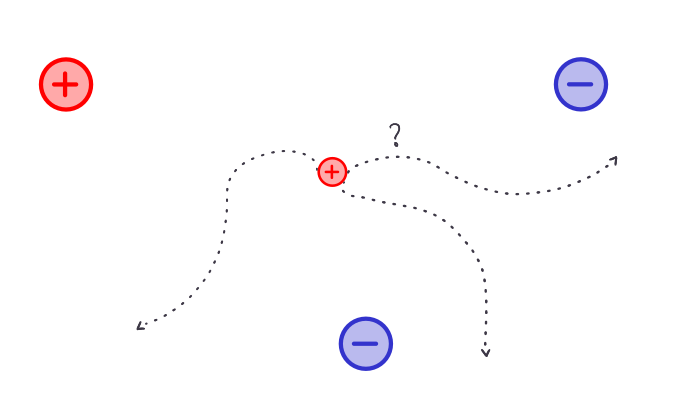
\includegraphics[width=0.5\textwidth]{images/field_ex_2.png}
    \caption{colocamos una cuarta carga en el centro y la soltamos.}
    \label{fig:campo_electrico_ejemplo_2}
\end{figure}


Para medir esta propiedad del espacio, imaginamos colocar una \hl{\textbf{carga de prueba positiva}} \( q^{+} \) en un punto del espacio y medir la fuerza que experimenta. Definimos el campo eléctrico como:

\begin{equation}
    \vec{E} = \frac{\vec{F}}{q}
    \label{eq:campo_electrico}
\end{equation}

donde:
\begin{itemize}
    \item \( \vec{E} \) es el campo eléctrico en ese punto,
    \item \( \vec{F} \) es la fuerza experimentada por la carga de prueba \( q \),
    \item \( q \) es la carga de prueba (se asume pequeña para no alterar el sistema).
\end{itemize}

\paragraph{¿Qué es la carga de prueba?}

La carga de prueba es una carga hipotética utilizada para medir el campo sin modificarlo. Debe cumplir dos condiciones:
\begin{enumerate}
    \item \textbf{Ser suficientemente pequeña} (\( q \to 0 \)): Así evitamos que su presencia afecte el sistema (es decir, que genere su propio campo que altere el original).
    \item \textbf{Ser positiva} por convención: Esto se hace para que el campo eléctrico tenga una dirección bien definida. Si el campo en un punto tiene dirección \textbf{hacia afuera}, significa que la carga fuente es positiva. Si el campo apunta \textbf{hacia adentro}, la carga fuente es negativa.
\end{enumerate}

\begin{figure}[ht]
    \centering
    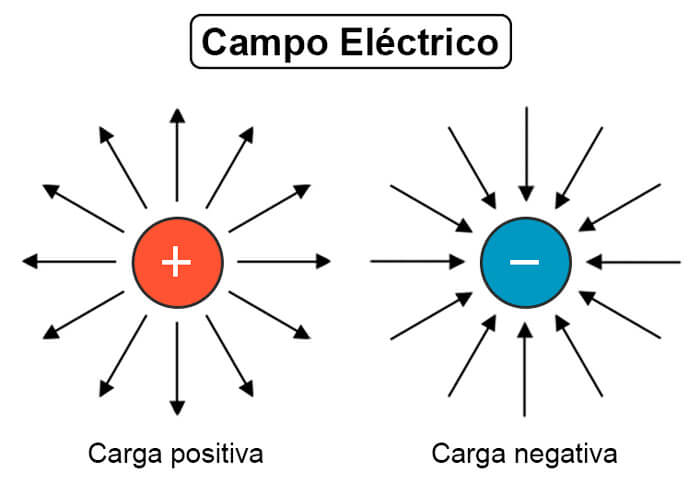
\includegraphics[width=0.5\textwidth]{images/electric_field.jpg}
    \caption{Campo eléctrico de una carga puntual positiva y una negativa.}
    \label{fig:campo_electrico}
\end{figure}

Si tomamos una carga fuente \( Q \) en el vacío, y colocamos una carga de prueba \( q \), respetando la convención anterior, a una distancia \( r \), la Ley de Coulomb nos da la fuerza sobre \( q \):

\[
\mathbf{F} = k_e \frac{Q \cdot q}{r^2} \hat{\mathbf{r}}
\]

Para quitar la carga de prueba \( q \) podemos dividir por \( q \). Al hacer esto obtenemos el campo eléctrico generado por \( Q \):

\[
\mathbf{E} = k_e \frac{Q}{r^2} \hat{\mathbf{r}} = \frac{\mathbf{F}}{q}
\]

Este resultado nos dice que el campo eléctrico \textbf{se aleja} de cargas positivas y \textbf{se dirige hacia} cargas negativas. Además disminuye con el cuadrado de la distancia y es una propiedad del espacio ya no depende de la carga de prueba \( q \), sino solo de \( Q \).

**6. Premisas clave de la definición**
1. **La carga modifica el espacio circundante:** El campo eléctrico es una propiedad del espacio, no de la carga de prueba.
2. **El campo es independiente de la carga de prueba:** La carga de prueba se usa solo como herramienta de medición.
3. **El campo es un campo vectorial:** Tiene dirección y magnitud en cada punto del espacio.
4. **El campo sigue el principio de superposición:** Si hay varias cargas, el campo total en un punto es la suma vectorial de los campos generados por cada una.

---

Este es el punto de partida. ¿Quieres que exploremos más sobre la deducción de otras ecuaciones o la aplicación a casos específicos?

El campo eléctrico \( \vec{E} \) es una propiedad del espacio que rodea a una carga y se define como:

\begin{equation}
    \vec{E} = \frac{\vec{F}}{q}
\end{equation}
